% Chapter 2

\chapter{Gestion de projet} % Main chapter title

\label{Chapter2} % For referencing the chapter elsewhere, use \ref{Chapter2} 

%----------------------------------------------------------------------------------------

\section{Organisation de l'équipe}

\subsection{Membres du projet}

\begin{table}[htp]
    \centering
    \begin{tabular}{|p{0.3\textwidth}|p{0.6\textwidth}|}
        \hline
        \tabhead{Nom / Prénom & Rôle}
        \hline
        Patrick \textsc{Piquart} & Scrum Master : Responsable de l'organisation interne et de la communication avec le client \\ \hline
        David \textsc{Coué} & Product Owner : Responsable de la communication avec le client \\ \hline
        Alan \textsc{Ait-Ali}  & Développeur \\ \hline
        Martin \textsc{Laporte} & Développeur \\ \hline
        Clément \textsc{Ailloud} & Développeur \\ \hline
        Romain \textsc{Petit} & Développeur \\ \hline
    \end{tabular}
    \caption{Membres du projet} \label{tab:membres} 
\end{table}

\subsection{Organisation externe}

À l’initiative de ce projet, il s’est tenu une présentation pour les sections Master 1 et Master 2 de
la formation. À l’issue de celle-ci, M. David Coué et M. Patrick Picard ont formé un groupe de 4
étudiants. Initialement, M. Patrick Picard a pris le rôle de “Scrum Master”, c’est avec lui que s’est
faite la “kick-off review”. Une réunion a ensuite eu lieu pour que le groupe de travail puisse bien
cerner les enjeux et qu’il soit en accord sur les méthodes de suivi de projet. Matérialisé par un
“backlog product”, cette méthode a permis d’avoir une bonne communication interne et de suivre 
l’avancement des différentes tâches. Pour la communication avec le client, le groupe d'étudiant
devait impérativement passer par  le “Product Owner” ou le “Scrum Master” pour faire remonter les
informations. \medskip

Quelques temps après la “kick-off review", le groupe de travail rencontra les ingénieurs en charge
du projet. À l’occasion de cet entretien fut exposé l’état de l’art ainsi que des avis sur certains
points techniques. \medskip

L’emploi du temps du projet et celui du Scrum Master n’étant pas compatible, les “daily review” se
sont tenues quasi-quotidiennement jusqu’à fin décembre entre les 4 étudiants. Face à la désinformation
du “Scrum Master” et des clients, un changement de méthode nous a été conseillé en janvier. La daily
fut alors remplacée par un rapport d’avancement. Cette méthode a permis de renouer le lien entre le
travail fournit par les étudiants et le client. Cela a fait prendre une toute nouvelle direction au
projet, malheureusement un peu tard car le projet devra s'arrêter le 25 février.\medskip

La gestion du partage des tâches au sein de l’équipe s’est auto-organisée selon les tâches à
développer. On ne pourra pas attribuer de rôle bien précis à chacun car en fonction de l'avancée du
projet les rôles se sont intervertis.

\begin{figure}[th]
    \centering
    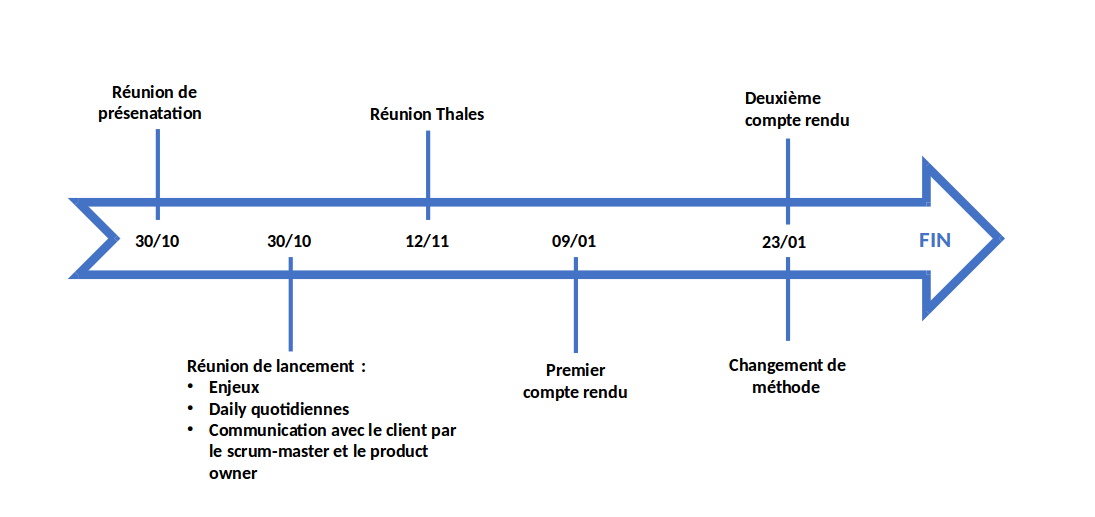
\includegraphics[scale=0.35]{Figures/fleche.png}
    \decoRule
    \caption{Chronologie du projet}  \label{fig:fleche}
\end{figure}

\subsection{Organisation interne}

À l’initialisation du projet, nous avons décidé de nous séparer en deux groupes. Le
premier groupe portera son étude depuis la couche haut niveau. À l’inverse, le second
groupe partira du bas niveau (modèle OSI). Pour mieux appréhender les différents
problèmes et axes de développement dans leur ensemble. \medskip

Le binôme Clément et Romain recherchaient à faire le lien depuis les couches applicatives
vers le kernel. Le binôme Alan et Martin au contraire cherchaient à établir en priorité les
couches basses pour ensuite les rendre compatibles avec le kernel.
Pour résumer les deux binômes n’avaient pas le même point de départ tout en ayant le
même kernel comme point d’arrivée. Clément et Romain sont donc chargés de
comprendre l’utilisation de Gstreamer et de la couche V4L2 ; Martin et Alan de rendre les
drivers compatibles avec notre système.  \medskip

Afin de se concentrer sur l’option la plus prometteuse (c.f. imx219 - Nvidia-Tegra
Chromium-Os) nous nous sommes lancés dans l’analyse du code C du pilote, donc
de son fonctionnement interne. Le code réparti entre chacun, nous avons cherché à
comprendre les utilités des structures et de l’organisation du code. Nous
avons poursuivi les appels aux fichiers systèmes, en mutualisant les informations
oralement. Grâce à cette organisation agile nous avons pu préciser la source du problème
avant d’en chercher la solution.  \medskip

Par la suite Romain et Alan se sont lancés dans le second objectif d’évolution. Ils ont
compilé un noyau linux récent, afin de précéder le portage des sources spécifiques à la
carte de développement (board support package, BSP) Openrex de la distribution.
En raison du peu de résultats et des nouvelles pistes données par le client, le groupe s’est
orienté vers l’étude d’un driver existant. Chacun est chargé de comprendre et modifier les
fonctions pour les rendre compatibles avec notre camera.  \medskip

En clair, le groupe s'est organisé de façon à progresser le plus rapidement possible sur
une même piste. Au maximum, deux pistes différentes étaient étudiées en parallèle.
Lorsque le travail pouvait être divisé, chaque binôme s’occupait d’en prendre une partie
pour ensuite tout remettre en commun.

\section{Diagramme de Gantt}

\begin{figure}[!htb]
    \centering
    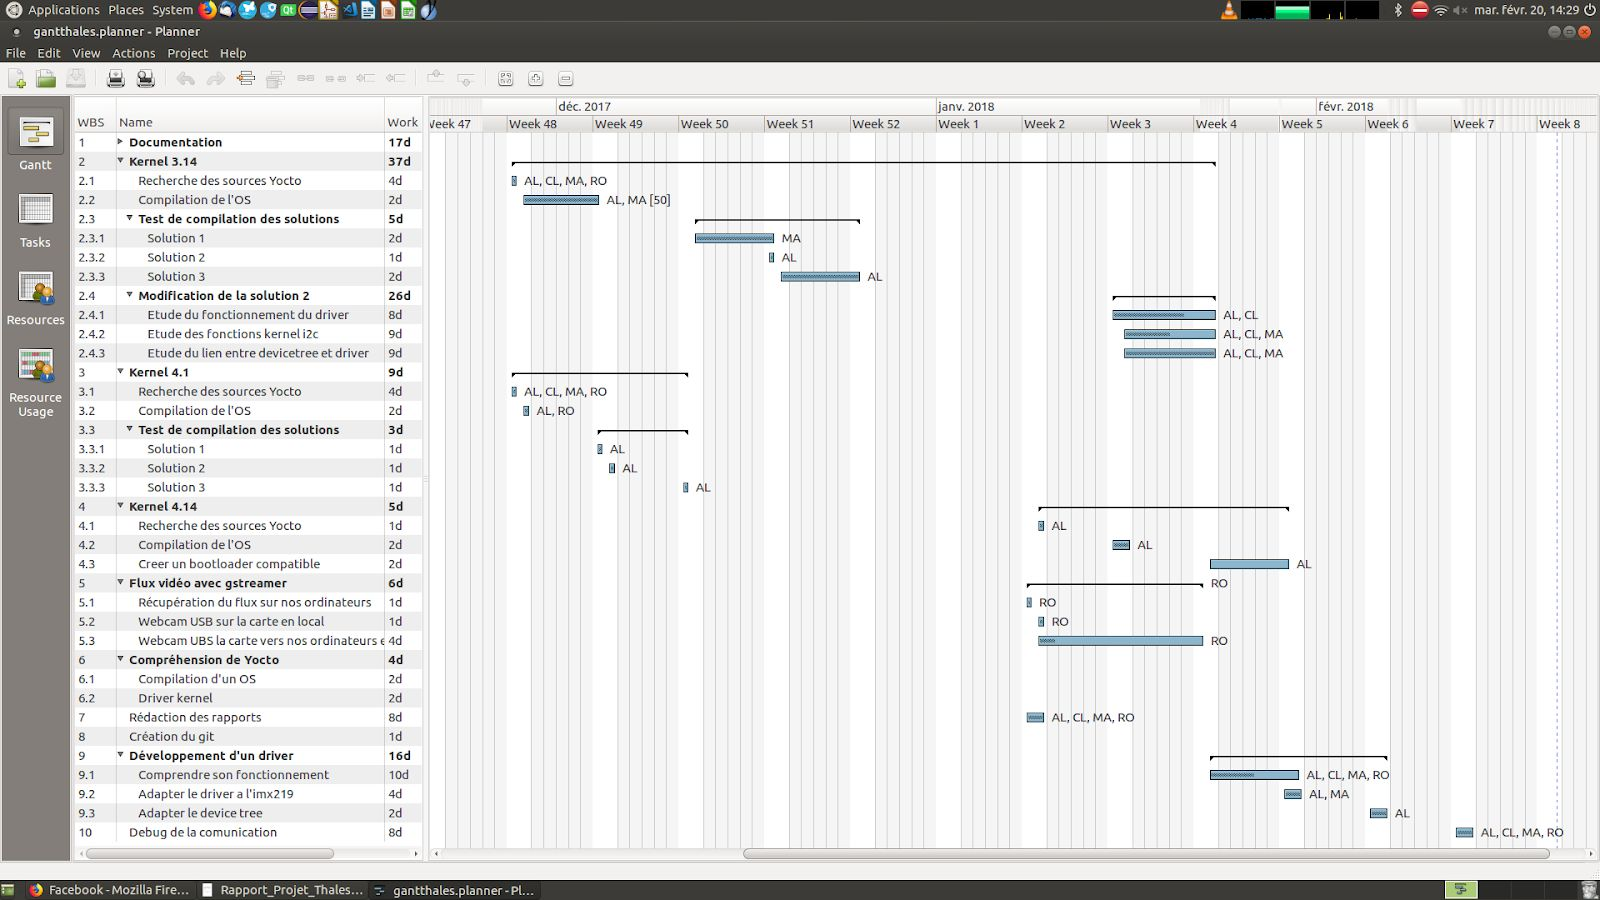
\includegraphics[angle=90,trim={2.5cm 2cm 0cm 3.5cm},clip,scale=0.35]{Figures/gantt.png}
    \decoRule
    \caption{Avancement détaillé du projet} \label{fig:planning}
\end{figure}

\clearpage

\section{Outils utilisés}

\subsection{Versionning des codes}

GitHub est un service de versioning ainsi qu’un service web d’hébergement. Il permet de
stocker toutes les sources d’un projet en différenciant par des versions. En effet, si nous
effectuons des modifications corrompant tout le projet, il est possible de récupérer la
version fonctionnelle si elle a été versionnée. \medskip

GitHub est trés utilisé dans le monde professionnel puisqu’il permet à plusieurs dizaines
de personnes à travailler simultanément sur un projet, par exemple le système
d’exploitation Linux sur GitHub mis à jour par des centaines de contributeurs. \medskip

Une fonctionnalité importante aussi est le système de “branches”. Si l’on souhaite séparer
certaines parties indépendantes d’un projet on utilise ce système. Cela permet de travailler
sur les mêmes fichiers en parallèle sans que les modifications apportées par les autres ne
posent de problèmes, à condition que les lignes concernées soient différentes. Le
versioning d’un projet s’effectue avec les quelques commandes principales ci-dessous.

\subsubsection{Commandes}

\begin{itemize}
    \item[Clone : ] Crée un dépôt local sur l’ordinateur depuis un dépôt en ligne
    \item[Add : ] Ajoute les fichiers ou dossiers dans l’index que nous voulons versionner sur le
    GitHub
    \item[Commit : ] Transfère le contenu de l’index vers le répertoire local ; commet la version. il est
    possible de rajouter un commentaire avec l’option -m
    \item[Push : ] Pousse les fichiers et dossiers contenus dans le répertoire local vers le dépôt en
    ligne après la commande commit
    \item[Pull : ] Actualise la branche locale sur l’ordinateur depuis un dépôt en ligne
    \item[Branch : ] Créé une nouvelle branche
    \item[Checkout ] Change de branche
    \item[Diff : ] Affiche les différences de fichiers entre le contenu local et le contenu du dépôt en
    ligne
\end{itemize}

Voic un shéma résumant graphiquement toutes les commandes ci-dessus :

\begin{figure}[!htb]
    \centering
    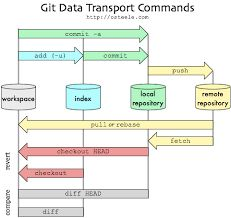
\includegraphics[trim={0cm 0cm 0cm 0cm},clip,scale=0.8]{Figures/git.png}
    \decoRule
    \caption{Résumé des commandes git} \label{fig:git}
\end{figure}

Il existe sur internet de nombreuses recommandations pour entretenir un dépôt git propre.
Étant débutants du principe, nous nous sommes concentrés sur l’aspect fonctionnel.

Ci-dessous, l’adresse de notre GitHub :

\href{https://github.com/Alanaitali/meta-openrexpicam}{https://github.com/Alanaitali/meta-openrexpicam}

\subsection{Communication}

A l’aube du projet quand nous avons choisi nos méthodes de communication, nous avons
décidé d'utiliser le logiciel (et hébergeur) de dialogue instantané nommé Slack. D’une part
nous avions déjà défini que nous nous verrions deux jours hebdomadairement d’autre part
nous avions déjà choisi de dialoguer avec l’équipe Thales en passant par notre
superviseur par mail qui relayerai les requêtes. Enfin comme précisé ci-dessus, un git
était à l’œuvre pour les échanges de code.

\subsubsection{Avantages de Slack}

\begin{itemize}
    \item[-] Interface très complète de dialogue en groupe
    \item[-] Capacité de rechercher parmi les messages
    \item[-] Conversations publiques/privées, en sous-groupe... etc
    \item[-] Accessible depuis un navigateur, et application pour ordinateur et smartphone de tous
    types, utile pour être notifié.
    \item[-] Gestions séparées des projets pour éviter de s’éparpiller sur un autre contenu (orientation
    professionnelle)
    \item[-] Appel à des applications en ligne possible (calc, github, google\_drive ...)
\end{itemize}

\subsubsection{Inconvénients de Slack}

\begin{itemize}
    \item[-] Gestion des logins indépendantes entre les projets (contre intuitif)
    \item[-] Applications mobiles et ordinateur non-native et donc plus consommatrices
    \item[-] Interface nouvelle avec des capacités restées inexploitées (planning, fils de discussions
    sur un message)
\end{itemize}

\subsection{Yocto}

OpenEmbedded, était à son commencement en 2003, un projet de la société du même
nom, rejointe plus tard par OpenZaurus. Avant son arrivée, l'outil massivement employé
était Buildroot, celui-ci étant principalement prévu pour construire des systèmes de fichiers
et non des distributions voire des SDK GNU-Linux. \medskip

En 2010 OpenEmbedded devient un “lab workgroup” de la fondation Linux avec 22
entreprises collaborant entre-elles. En 2011, lors de son rachat par Intel, le projet est
nommé Yocto. Celui-ci a pour but de faciliter la conception de systèmes Linux avec une
empreinte mémoire minime et la compilation croisée. Il permet théoriquement de
développer une distribution spécifique aux besoins d’un utilisateur indépendamment de la
cible et du poste de développement. \medskip

\clearpage

Enrichi par un grand nombre d’entreprises tel que NXP ou Texas instrument, le projet
Yocto s’est développé et est maintenant maintenu autour de deux blocs :

\begin{itemize}
    \item[-] Bitbake : outil de construction dérivé du gestionnaire de paquet “portage” par
    l’équipe du projet OpenEmbedded. Bitbake active les différents ingrédients utiles à
    la compilation des recettes.
    \item[-] OpenEmbedded-core : les sources de base sous forme de métadonnées pour la
    génération d’un système GNU/Linux base, la distribution poky.
\end{itemize}

Yocto peut être rendu compatible avec de très nombreuses combinaisons de SBC et SOM
grâce à une gestion open-source et à la méthode de développement incrémental des
recettes qu’il instaure. Il permet de générer une distribution complète (image, bootloader,
SDK, rootfs, device-tree...), à partir d’assemblages de métadonnées. À l’intérieur des
méta-données nous trouvons des recettes et des bouts de recettes dépendants d’une
recette mère. Une recette correspond à un arbre de compilation. \medskip

Bitbake se charge alors de parcourir (fetch) les sources pour recomposer la recette à travers le 
fichier .bb et les fichiers .bbappend dans un arbre de compilation, puis exécute la compilation.
Cela fait,  il installe tous les binaires dans une même image. L’un des principaux inconvénients de
Yocto, est le besoin de disposer d’un grand espace disque (environ 50 Gb). La première fois, Yocto
a conservé  plusieurs états des tâches. Ainsi, tout ce qui n’a pas été modifié ne sera pas exécuté
à nouveau par Bitbake, on gagne alors un temps précieux en échange de l’espace mémoire
(shared-state cache).

\subsubsection{Poky}

Poky c'est la distribution de référence générée par Yocto, elle est maintenue pour être
compilable sur toutes les machines cibles officielles et se compose :

\begin{itemize}
    \item[-] d'un bootloader (U-boot)
    \item[-] d’un Kernel Linux, et d’applications (GNU compilant pour la plupart)
    \item[-] d’un device tree (fichier binaire .dtb) qui peut être interprété dans /sys/ par des
    drivers
    \item[-] d’un système de fichiers partant du répertoire racine dit rootfs
    \item[-] d’éventuels modules et drivers
\end{itemize}

Poky contient concrètement les lignes de codes nécessaires à l'obtention d'une distribution.

\subsubsection{Bitbake}

Bitbake est un outil de compilation de sources à partir de répertoires locaux et en ligne. Il
décompose chaque phase de compilation en : do\_fetch, do\_unpack, do\_patch,
do\_configure, do\_compile, do\_install, do\_package. Une caractéristique essentielle de
Bitbake est sa capacité à gérer les interruptions dans la compilation et de pouvoir
reprendre la compilation là où il l'avait laissé, à un tâche prête.
Les étapes do\_fetch et do\_unpack respectivement, téléchargent et décompressent les
sources vers le répertoire de travail (variable \$WORKDIR). Pour cela ils passent par un
répertoire intermédiaire de téléchargement (\$DL\_DIR), ces sources peuvent être
téléchargées à la demande par une commande, telle que celle ci-dessous, pour le packet
zlib. En effet, pour des problèmes de connexion réseau, il peut être nécessaire de
déclencher manuellement le téléchargement des paquets non récupérés.

\begin{tcolorbox}
    user@poky:~/fsl-community-bsp/build\$ Bitbake -c fetch zlib
\end{tcolorbox}

Les étapes do\_configure et do\_compile correspondent à la préparation de l'arborescence
de compilation et à la compilation même (précompilation, ln, as...)
des recettes qui composeront l’image. Bitbake sous-traite la préparation et la
compilation sur des commandes comme autotools, cmake, scon, qmake ou encore un
script « ./configure », make, make install; ce choix étant laissé aux rédacteurs du paquet.

Alors que la commande make se contente de placer le fichier Makefile pour ordonner les
compilations, Bitbake apporte plus de dynamisme. Les ordres d’une compilation Bitbake
sont décentralisés sur 3 formats de fichiers. Principalement les .bb sont les fichiers «
recette-mère » qui seront parcourus par Bitbake et déclencheront la compilation (ou non)
des sources en présence. Les fichiers .bbappend (recette-fille) permettent de compléter un
fichier .bb, et les fichiers .bbclass permettent d’indiquer a Bitbake de prendre en compteles
.bb et .bbappend. L'intérêt étant de classer les recettes mères et filles dans des
dossiers (métadonnées ou meta) par fonctionnalité et non par dépendance de compilation.
En constant développement, le “projet Yocto” se compose de poky, Bitbake, ainsi que
l’ensemble des métadonnées mises à disposition par la communauté.

\section{Caméra Raspberry Pi v2}

\begin{figure}[!htb]
    \centering
    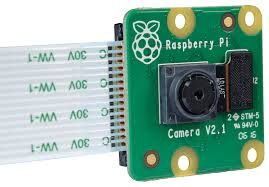
\includegraphics[trim={0cm 0cm 0cm 0cm},clip,scale=0.4]{Figures/camrpi.png}
    \decoRule
    \caption{Raspi Cam v2} \label{fig:camrpi}
\end{figure}

La Raspberry Pi Caméra (V2) est la dernière version de la gamme Raspberry. Cette
caméra dispose d’un microcontrôleur imx219 développé par Sony. C’est un composant
d’acquisition d’images associé à un système optique et à quelques composants passifs.
Pour donner une notion de ses capacités, ce microcontrôleur est capable de réaliser une
capture vidéo 1080p à 60 images/s. \medskip

Dans le document suivant nous parlerons toujours du driver imx219 pour désigner le driver
de la caméra Raspberry Pi. La communication avec l’imx219 se fait à travers l’utilisation
de l’I2C sur port CSI2 disposant d’une connexion D-phy 2 ou 4 Lanes et d’une clock pour
le transfert du flux vidéo. Dans notre cas, nous travaillons avec la configuration 2 lanes. La
connexion utilise donc 6 broches avec un doublet (une lane) de pistes en communication
half-duplex et les 2 autres doublets en simplex.\medskip

L’utilisation de l’interface I2C permet de configurer les registres de l’imx219 et de
récupérer le flux vidéo. la communication se fait à une fréquence comprise entre 11 MHz
et 27 MHz.\medskip

Enfin la présence de la broche XCLR permet le reset du composant.
De la documentation technique est accessible pour l’imx219, cependant nous n’avons pas
trouvé la schématique de la carte caméra Raspberry .

\section{Interface caméra MIPI CSI-2}

L’alliance MIPI compte plus de 250 entreprises aujourd’hui mais parmi les 6 contributeurs
initiaux (02/2004) on compte ARM limited, NXP Semiconductors et OmniVision
Technologies AG. Ce dernier est également producteur de contrôleur-caméra. Nous
reparlerons plus tard du composant ov5640 car celui-ci est déjà présent sur la plateforme
openrex au kernel 4.1. \medskip

L’interface processeur des industriels du mobile
standardise les communications avec tous lespériphériques habituels environnant le processeur d’un smartphone. Pour accéder à une
caméra l’interface prévoit une communication par le protocole CSI ou CSI-2 et une liaison
par les couches physiques C-phy et D-phy (M-phy étant en développement). Ce genre de
connexion s’effectue avec 2 à 4 lanes de données et une lane d’horloge. Une lane est un
même signal différentiel à haute fréquence. Dans le standard D-phy, une lane
d’information est transportée sur deux pistes électroniques (en différentiel). Dans le
standard C-phy, 2 lanes d’information peuvent transiter sur 3 pistes électroniques
(doublement différentielles), mais nous ne nous intéresserons pas au C-phy. \medskip

Cette illustration présente les différentes “lane” du block MIPI :

\begin{figure}[!htb]
    \centering
    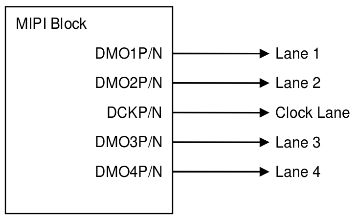
\includegraphics[trim={0cm 0cm 0cm 0cm},clip,scale=0.4]{Figures/blockMIPI.png}
    \decoRule
    \caption{Différents signaux du MIPI} \label{fig:blockmipi}
\end{figure}

L’imx6s Openrex supporte le mode M-phy 2 lanes. Les deux broches de données et la
broche de la clock seront respectivement les broches (DMO1P/N, DMO2P/N, DCKP/N) du
port CSI-2.

\section{Carte de développement OpenRex}

\begin{figure}[!htb]
    \centering
    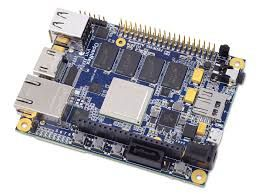
\includegraphics[trim={0cm 0cm 0cm 0cm},clip,scale=0.55]{Figures/openrex.png}
    \decoRule
    \caption{Carte OpenRex Basic} \label{fig:openrex}
\end{figure}

L’Openrex est une carte de développement conçue par Fedevel et produite par Voipac.
Elle intègre un « système on chip » IMX6 disposant de un ou quatre coeurs suivant les
versions. La schématique ainsi que le routage de ces deux cartes sont opensources et
disponible sur le site de \href{http://www.imx6rex.com/open-rex/}{http://www.imx6rex.com/open-rex/}.


Notre objectif est de porter le driver imx219 de la Raspberry sur l’IMX6S Openrex. Cette
dernière possède un port CSI-2 identique au port de la Raspberry Pis. De plus, ce port peut accueillir des niveaux de tensions LVDS, nous avons donc vérifié qu’elle était
configurée sur le port CSI-2 comme indiqué par la figure X. Le routage du connecteur
correspond donc à la figure XX? On y retrouve les couples de pistes lane D0, lane D1 et la 
CLK0, les deux broches de communication I2C SCL et SDA, les deux GPIO.

\section{Video for Linux 2 (V4L2)}

V4L2 est la seconde version de l’API V4L. Elle est utilisée par des périphériques vidéo
(caméras, écrans) contenue dans l’espace utilisateur d’un système linux. Elle est aussi
faite de composants audio contrôlés par l’API Alsa. Elle permet de manipuler une très
grande variété de périphériques en utilisant les mêmes fonctions. En général, il s’agit de
périphériques I2C, mais si ce n’est pas le cas, une structure (v4l2\_subdev) a été créée
pour fournir au driver une interface en adéquation avec celle des sous-périphériques.

Principe d'usage :

\begin{itemize}
    \item[-] Ouvrir le périphérique
    \item[-] Modifier les propriétés de l'appareil (résolution, luminosité, ...)
    \item[-] Sélectionner le format de donnée
    \item[-] Récevoir / Envoyer les données
    \item[-] Ferme le périphérique
\end{itemize}

Les drivers V4L2 sont implémentés comme des modules kernels, ils sont chargés
automatiquement ou manuellement (suivant les drivers) lors de la détection du
périphérique par le système. Ils s’exécutent dans le kernel-space c’est-à-dire sous le
kernel.

La commande ci-dessous est une surcouche de la commande insmod. insmod charge
simplement un module, tandis que modprobe charge ses modules dépendants également.

\begin{tcolorbox}
    root@poky:~\# modprobe <driver\_name>
\end{tcolorbox}

Suite au chargement du module, le gestionnaire de périphériques “udev” va créer un
fichier dans le répertoire /dev, permettant ensuite l’accès aux périphériques. Selon le choix
au développement, une arborescence de contrôle plus poussée peut apparaître dans /sys.

\subsection{Package V4L-utils}

Aujourd'hui le package v4l-utils implémente V4L2 dans une distribution , V4L devenant obsolète.

\subsection{Principales commandes de contrôle}

\begin{itemize}
    \item[v4l2-ctl : ]  outil de contrôle utilisé en ligne de commande
    \item[v4l2-dbg : ] outil permettant l'accés aux registres des périphériques v4l2
    \item[q4l2 : ] interface graphique v4l2 utilisant les commandes de contrôle de l'API
\end{itemize}

\begin{figure}[!htb]
    \centering
    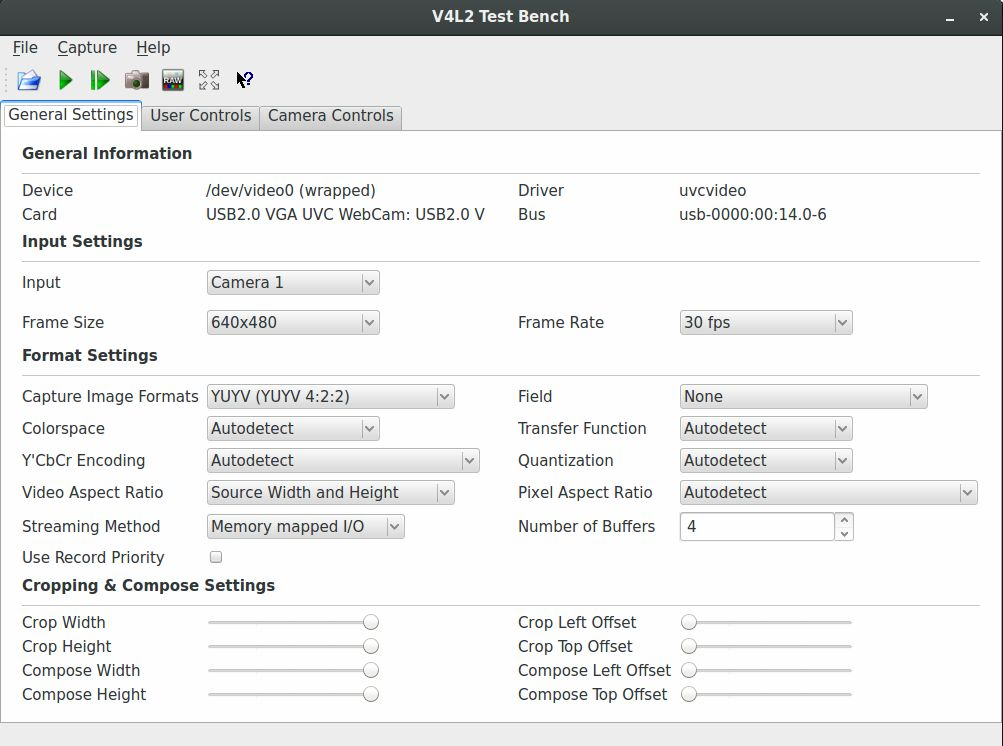
\includegraphics[trim={0cm 0cm 0cm 0cm},clip,scale=0.35]{Figures/v4l2.png}
    \decoRule
    \caption{Application graphique de V4L2} \label{fig:v4l2}
\end{figure}

L’API V4L2 met à disposition le package “v4l-utils”. Ce package fournit une interface
graphique et des commandes de contrôle permettant la configuration d’un périphérique. \medskip

Comme il est illustré sur la figure \ref{fig:v4l2}, cette interface permet la configuration
de  plusieurs paramètres disponibles sur une majorité des périphériques vidéo. \medskip

Paramètres généraux : sélection du périphérique d'entrée, configuration du format des données et
dimensionnement de l'affichage.

\begin{itemize}
    \item[Utilisateur : ] Configuration du rendu vidéo
    \item[Caméra : ] Configuration de l'exposition lumineuse
\end{itemize}

Pour manipuler l'ensemble de ces paramètres, les différentes structures de v4l2 doivent
être correctement instanciées dans le driver par les fonctions C, configurant la caméra.

\subsubsection{Structures V4L2}

\textbf{v4l2\_subdev}

\begin{lstlisting}
    struct v4l2_subdev
    {
        #if defined(CONFIG_MEDIA_CONTROLLER)
        struct media_entity entity;
        #endif
        struct list_head list;
        struct module * owner;
        bool owner_v4l2_dev;
        u32 flags;
        struct v4l2_device * v4l2_dev;
        const struct v4l2_subdev_ops * ops;
        const struct v4l2_subdev_internal_ops * internal_ops;
        struct v4l2_ctrl_handler * ctrl_handler;
        char name[V4L2_SUBDEV_NAME_SIZE];
        u32 grp_id;
        void * dev_priv;
        void * host_priv;
        struct video_device * devnode;
        struct device * dev;
        struct device_node * of_node;
        struct list_head async_list;
        struct v4l2_async_subdev * asd;
        struct v4l2_async_notifier * notifier;
        struct v4l2_subdev_platform_data * pdata;
    };
\end{lstlisting}

Cette structure permet de gérer le multiplexage audio et vidéo de
sous-périphériques (capteurs et contrôleurs de caméra).

\textbf{i2c\_client}

\begin{lstlisting}
    struct i2c_client
    {
        unsigned short flags;
        unsigned short addr;
        char name[I2C_NAME_SIZE];
        struct i2c_adapter * adapter;
        struct device dev;
        int irq;
        struct list_head detected;
        #if IS_ENABLED(CONFIG_I2C_SLAVE)
        i2c_slave_cb_t slave_cb;
        #endif
    };
\end{lstlisting}

Cette structure donne accès au bus i2c pour établir la communication et interagir avec le
périphérique. Pour protéger en écriture cette configuration, il est conseillé d’utiliser la
fonction v4l2\_set\_subdevdata(). Elle permet de stocker le pointeur de cette structure dans
les données privées de v4l2\_subdev.

\textbf{Initialisation de v4l2\_subdev}

Déclaration des fonctions d’initialisation dans la structure v4l2\_subdev\_core\_ops

\begin{lstlisting}
    static struct v4l2_subdev_core_ops imx219_subdev_core_ops =
    {
    .s_power = imx219_s_power,
    };
\end{lstlisting}

Implémentation des fonctions permettant l’initialisation des paramètres du flux vidéo :

\begin{lstlisting}
    static struct v4l2_subdev_video_ops imx219_subdev_video_ops = 
    {
    .s_stream = imx219_s_stream,
    .cropcap = imx219_cropcap,
    .g_crop = imx219_g_crop,
    .s_crop = imx219_s_crop,
    .enum_mbus_fmt = imx219_enum_mbus_fmt,
    .g_mbus_fmt = imx219_g_mbus_fmt,
    .try_mbus_fmt = imx219_try_mbus_fmt,
    .s_mbus_fmt = imx219_s_mbus_fmt,
    .g_mbus_config = imx219_g_mbus_config,
    };
\end{lstlisting}

On crée donc la structure du périphérique (imx219.c) :

\begin{lstlisting}
    struct <chipname>_state 
    {
        struct v4l2_subdev sd;
    };
\end{lstlisting}

Cette structure doit contenir la structure v4l2\_subdev pour donner un accés direct à la
configuration du sous-périphérique (interface i2c).

Initialiser le sous-périphérique i2c :

\begin{lstlisting}
    v4l2_i2c_subdev_init(&state->sd, client, subdev_ops);
\end{lstlisting}

Faire le lien entre la structure i2c et v4l2\_subdev :

\begin{lstlisting}
    struct i2c_client *client = v4l2_get_subdevdata(sd);
    struct v4l2_subdev *sd = i2c_get_clientdata(client);
\end{lstlisting}

Instancier la structure pour ajouter la configuration du périphérique au kernel :

\begin{lstlisting}
    struct v4l2_subdev * v4l2_i2c_new_subdev(struct v4l2_device * v4l2_dev, struct
    i2c_adapter * adapter, const char * client_type, u8 addr, const unsigned short *
    probe_addrs);
\end{lstlisting}

Charge la configuration du flux vidéo du port CSI-2 définit par l’utilisateur.

\begin{lstlisting}
    v4l2_subdev_video_ops->s_stream()
\end{lstlisting}

Mise sous tension du port CSI-2 :

\begin{lstlisting}
    v4l2_subdev_core_ops->s_power()
\end{lstlisting}

\section{GStreamer}

GStreamer est un framework multimédia développé en C et porté sur plusieurs autres
systèmes d’exploitation que GNU/Linux comme Android, OS X, iOS ou encore Windows.
Ce projet débuta en Juin 1999 et fut implémenté dans l’environnement bureautique
GNOME en Juillet 2012. \medskip

GStreamer utilise principalement des tubes (pipeline) inter-connectés ainsi le type d’un
flux traversant un tube est connu des autres de plus ce framework est capable de gérer
des fichiers audio et vidéo (capture, encodage, streaming, écoute, affichage).\medskip

GStreamer est basé sur des plugins qui améliorent son développement et ajoute des
fonctionnalités comme l’encodage/décodage géré par le plugin FFMPEG.\medskip

GStreamer propose une fonctionnalité de streaming en local ou par un réseau, cette
dernière passe par les protocoles UDP et TCP de la couche IP.\medskip

Le principe de ce framework repose sur l’association d’éléments reliés par des pipelines
cependant l’entrée d’un élément doit être compatible avec la sortie de l’élément précédent.
L’ordre des éléments est donc très important lorsqu’on écrit la commande, voici un
schéma expliquant l’ordre des éléments :

\begin{figure}[!htb]
    \centering
    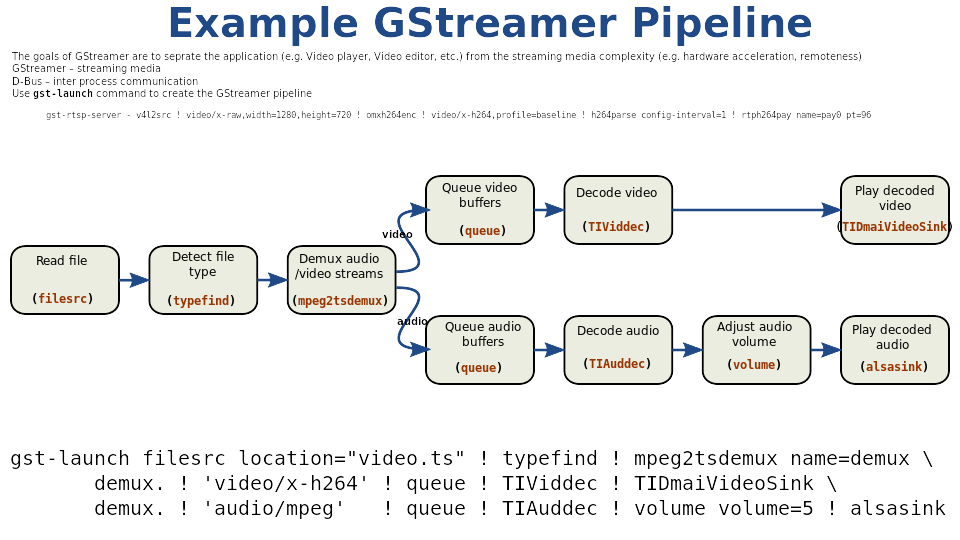
\includegraphics[trim={0cm 5cm 0cm 6cm},clip,scale=0.35]{Figures/gstreamer.png}
    \decoRule
    \caption{Étapes de GStreamer} \label{fig:gstreamer}
\end{figure}

La première étape indique la source de la commande GStreamer. Cela peut être un fichier
ou bien une caméra par le biais de V4L2. Ensuite, le système détecte le type du fichier
source et différencie un fichier audio d’un fichier vidéo.
Nous nous intéresserons plus sur la partie vidéo qu’audio puisque l’objectif du projet est la
capture du flux vidéo, pour cela nous allons expliquer les commandes que nous utilisions :

\begin{tcolorbox}
    user@poky:~\$ gst-launch-1.0 v4l2src ! 'image/jpeg,width=1280,height=720,
    framerate=30/1' ! imxvpudec ! imxipuvideotransform ! imxeglvivsink sync=false
\end{tcolorbox}

Si l’on souhaite visualiser le flux vidéo d’un appareil V4L2 avec la synchronisation
désactivé en 30 FPS et d’une résolution de 1280x720 pixels avec un format d’image
JPEG, cette commande est adaptée. De plus celle-ci utilise une synchronisation EGL ainsi
qu’un décodage V4L2.

\begin{tcolorbox}
user@poky:~\$ gst-launch-1.0 v4l2src ! 'image/jpeg,width=1280,height=720,
framerate=30/1' ! v4l2sink sync=false
\end{tcolorbox}

Cette commande permet d’afficher le flux vidéo de V4L2 en 30 FPS avec une taille de
1280x720 pixels. Si l’on souhaite juste faire une capture photo, l’image sera au format
JPEG. V4L2sink est utilisé pour afficher le flux vidéo de l’appareil V4L2 en désactivant la
synchronisation.

\begin{tcolorbox}
user@poky:~\$ gst-launch-1.0 v4l2src device=/dev/video0 ! 'image/jpeg,
width=1280,height=720, framerate=30/1' ! v4l2sink sync=false
\end{tcolorbox}

Cette commande est la même que la première, la seule différence vient de la source.
Celle-ci prend l’appareil vidéo numéro 0 en entrée qui correspond à la caméra.